\documentclass{article} % For LaTeX2e
\usepackage{final_project,times,graphicx}
%\documentstyle[nips12submit_09,times,art10]{article} % For LaTeX 2.09


\title{Predicting the Impact of Research Papers in the Covid-19 Open Research Dataset}



\author{
Tyler Ashoff \\
Department of Interdisciplinary Data Science\\
Duke University\\
Durham, NC 27708 \\
\texttt{ashofftyler@gmail.com} \\
\\
\textbf{Jennifer Wilson} \\
Department of Statistical Science\\
Duke University\\
Durham, NC 27708 \\
\texttt{jennifer.wilson994@duke.edu} \\
}

\newcommand{\fix}{\marginpar{FIX}}
\newcommand{\new}{\marginpar{NEW}}

\nipsfinalcopy

\begin{document}


\maketitle



\begin{abstract}
The volume of research papers and articles relating to Coronaviruses combined with the rapid increase at which new information is being published makes it nearly impossible for those relying on this research to keep up [1]. We propose the use of citation count prediction [2] to identify impactful articles which may have been overlooked.
\end{abstract}

\section{Introduction}

As the world community became engulfed in the Covid-19 pandemic in early 2020, the scientific community sprang into action. The rate at which new results and research are still being published is startling. In an effort to help identify potentially influential research, we turn to citation count prediction.

Citation count prediction is one of a number of methods for predicting the importance and popularity of a paper [2]. While numerous modeling methods have already been produced to predict this, we look at citation count prediction specifically as it relates to the Covid-19 Open Research Dataset (CORD-19) [1]. This dataset compiled by the Whitehouse and leading researchers provides information on over 57,000 articles, including the full text. This dataset provides some unique challenges related to the steep rise in articles recently published resulting in a dataset that is highly skewed. Additionally, the does not include information heavily relied on for citation count prediction such as the h-index [3]. Therefore we focus on extracting data from the documents and abstracts themselves in an attempt to predict citation count. Numerous different modeling techniques were attempted, including neural nets, zero-inflated poisson regression, hierarchical modeling and gradient boosting. Many of these models had little to no significance. 

\section{Data Wrangling}

The CORD-19 dataset is a collection of scientific articles about COVID-19, SARS-CoV-2, and related coronaviruses. Our 12,372 sample subset of this dataset is chosen by first selecting observations available on the NCBI website and second ensuring that the full body of the text is available in the dataset. Unfortunately citation data was not supplied in the CORD-19, to gather these values we scraped available citation data from the NCBI website. The information available in our compiled dataset included, journal of publication, full article text, authors, number of articles cited in the text, and number of citations received by the article. Since we are interested in understanding paper importance in terms of contribution to the field, these citations are key to our inquiry.

To transform the articles' text into usable features, each abstract and text body are run separately through gensim's python implementation of Doc2Vec. This resulted in a 100 dimensional vectorization of each text. We chose to analyze the abstracts independently because they are designed as a succinct summarization of the paper's content and could help focus the vectorization. Each of these vectorizations were then embedded into five dimensional space using a variational autoencoder, Isomap, and Spectral embedding. Using these embedded documents, we create three new features for the abstracts and the full text: mean Euclidean distance of five nearest neighbors, mean Euclidean distance of five nearest neighbors from the preceding six months, and a count of texts within an open ball of radius $0.1 * $\textit{standard deviation of all distances}. These were designed to measure where the work sits within the topic's literature, where it sits in relation to prior work, and density of work in the specific topic respectively. The final features used in the model are as shown in Figure \ref{features}.

\begin{figure}[h]
\begin{center}
  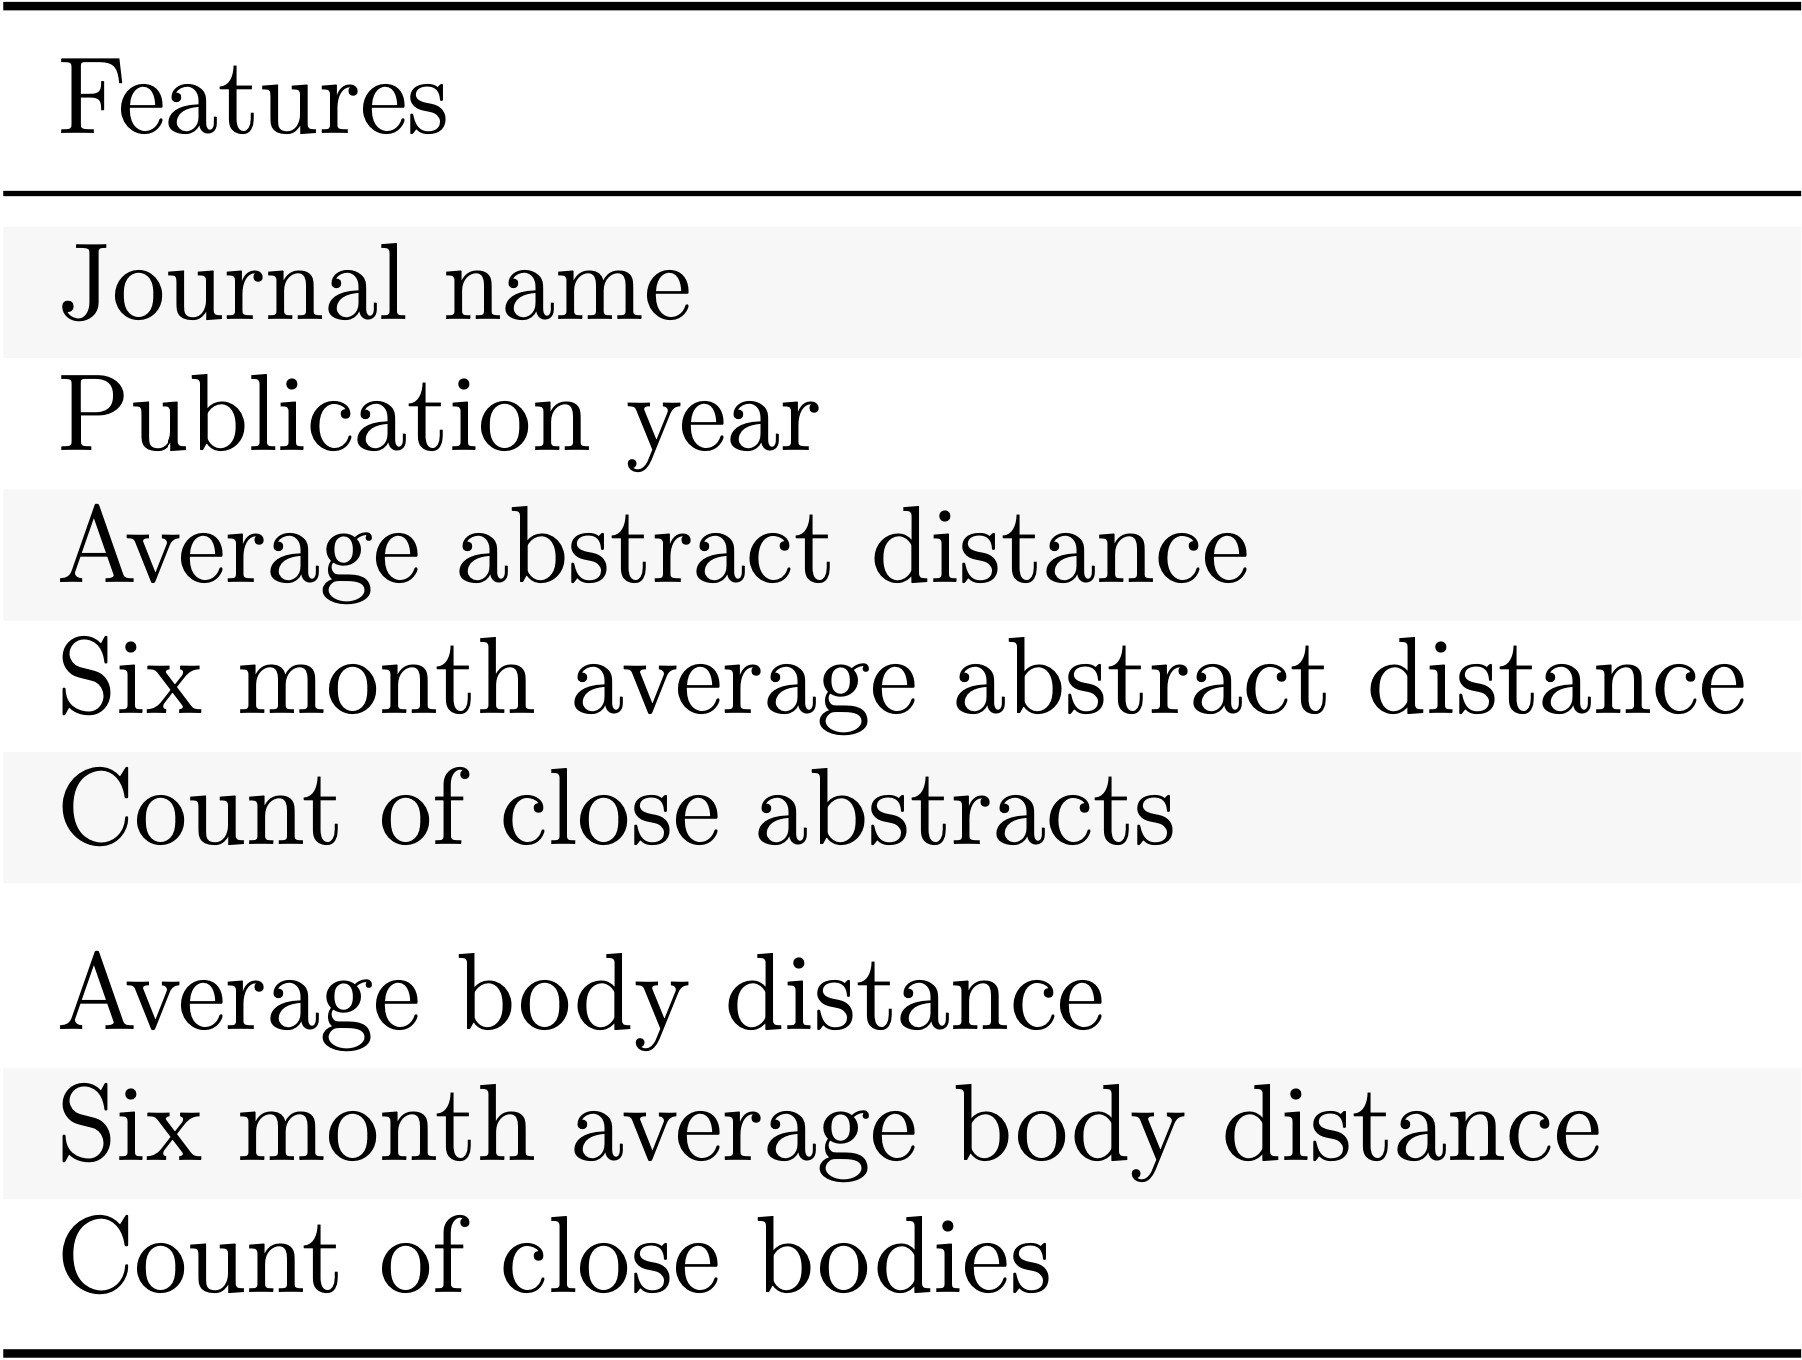
\includegraphics[scale=0.17]{../Figures/features.png}
\end{center}
\caption{Features included in analysis}
\label{features}
\end{figure}

Because our interest is in predicting paper influence for recent papers, we hold out all papers published in 2020. In addition to being the papers of interest, we felt the recent nature of their publication may have an influence on their total citation numbers. Our predicted ranking of these papers is reproduced in the appendices.



\section{Transformations}

Transformations of the response and covariates proved to have significant impact on model performance. Most gains in improving results came from transformations as opposed to tuning parameters.

\subsection{Response}
A significant number of articles in this dataset have no citations. While some of this is simply due to the fact that they have not been published long enough for others to have cited them yet, this phenomenon is still present when restricting to articles published in previous years. Additionally, there are some articles that receive a significantly large number of citations. We opt to use a $log(x+.01)$ transformation on the response which allows us to normalize the non zero counts and futher separate articles with citations from those without. While not among the final models we present, we did attempt a zero inflated poisson model without the transformation to try and deal with the high mass at zero. This model had poor results.


\begin{figure}[h]
\begin{center}
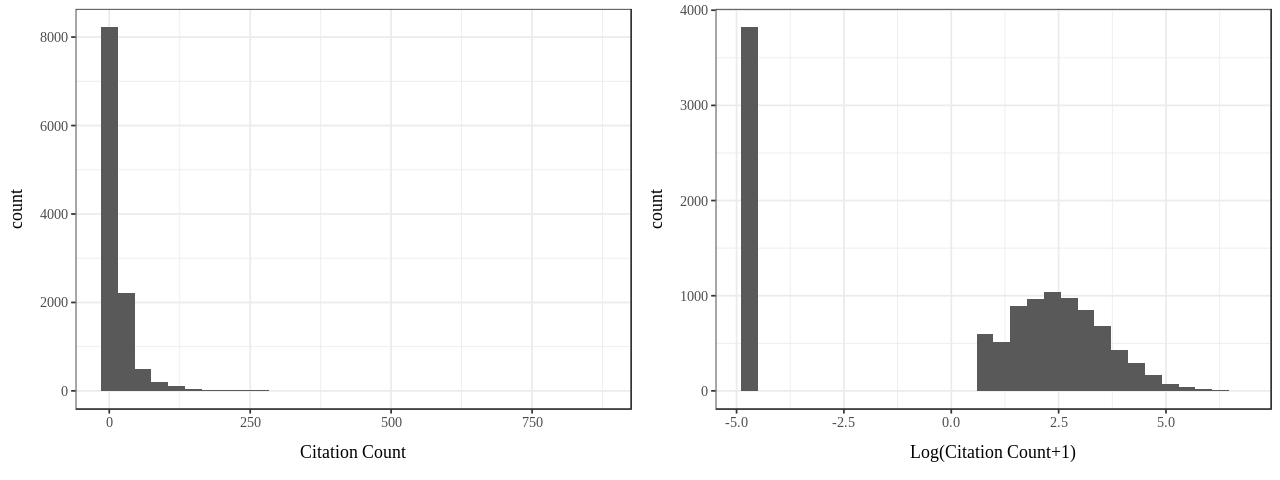
\includegraphics[scale=0.5]{../Figures/citation_hist.png} 
\end{center}
\caption{Transformation of Citation Count}
\end{figure}


\subsubsection{Covariates}
Many of the covariates from the embedding task were not linearly related to the citation counts. Most often this appeared as a high citation count and lots of density near a value of 0 with low citation counts in the positive and negative limits with low density. We use a $log(x^2)$ transformation of these covariates. While somewhat convoluted and uninterpretable, this transformation does a good job at spreading out the distribution of the data and linearizing the relationship. Additionally, a log transform is applied to the average abstract distance, six month average abstract distance, average body distance, and six month average body distance.


\section{Results}

The most successful model is an xgboost model with max depth of 5, learning rate of 0.5, and objective functions squared error and hinge loss for regression and binary classification respectively. Results from the xgboost model and a random forests model can be seen in Figures \ref{binary} and \ref{regression}. In addition to these models we tested linear models, a neural network, and Gaussian process regression and classification. However, the tree based methods performed best on the training data.

The results show that while the choice of embedding had an effect on accuracy, with the variational autoencoder embedding performing best, these improvements were only marginal. Similarly, the effect of the text based features, while helpful,  were less important than date of publication and journal of publication. Inspection of feature importance from the xgboost model showed that far and away the most predictive feature for citations is the journal in which the work is published.


\begin{figure}[h]
\begin{center}
  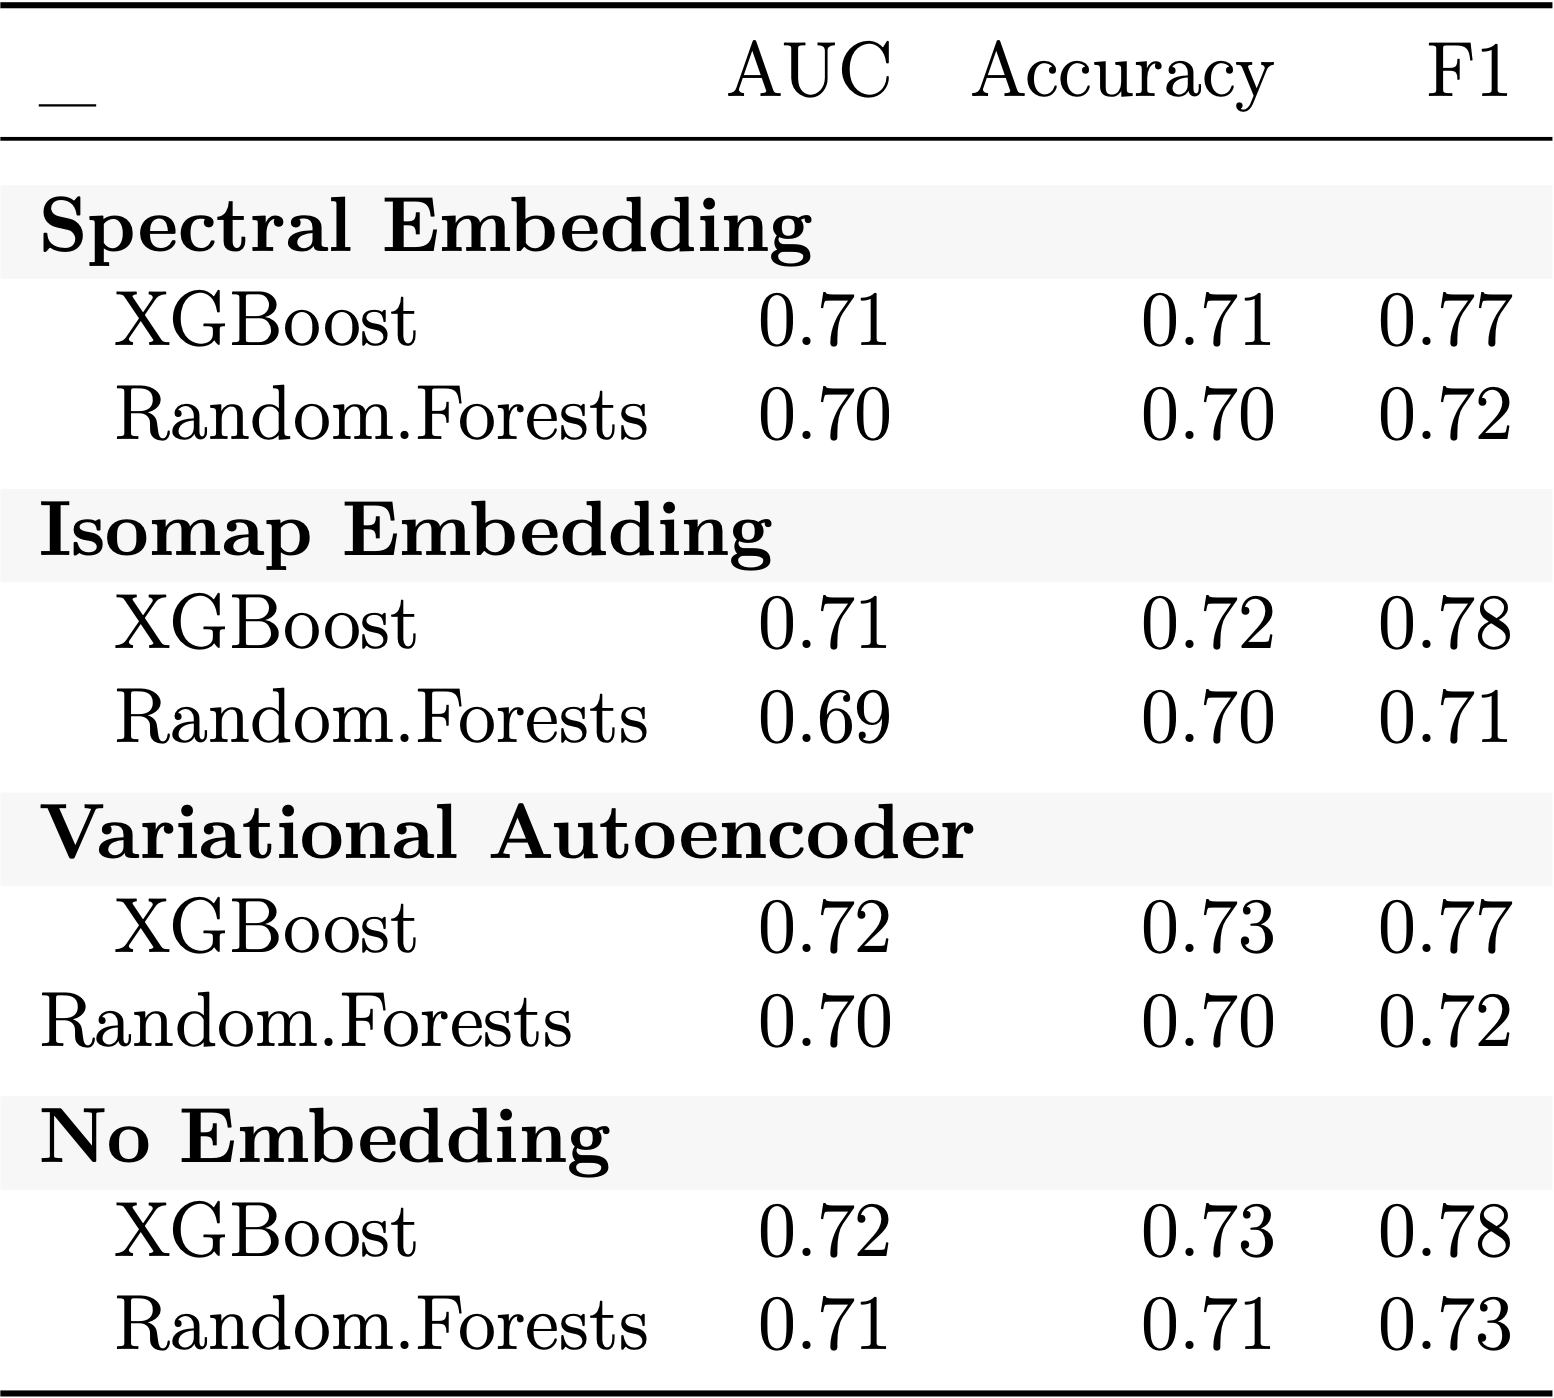
\includegraphics[scale=0.22]{../Figures/binary.png}
\end{center}
\caption{Binary Response}
\label{binary}
\end{figure}


\begin{figure}[h]
\begin{center}
  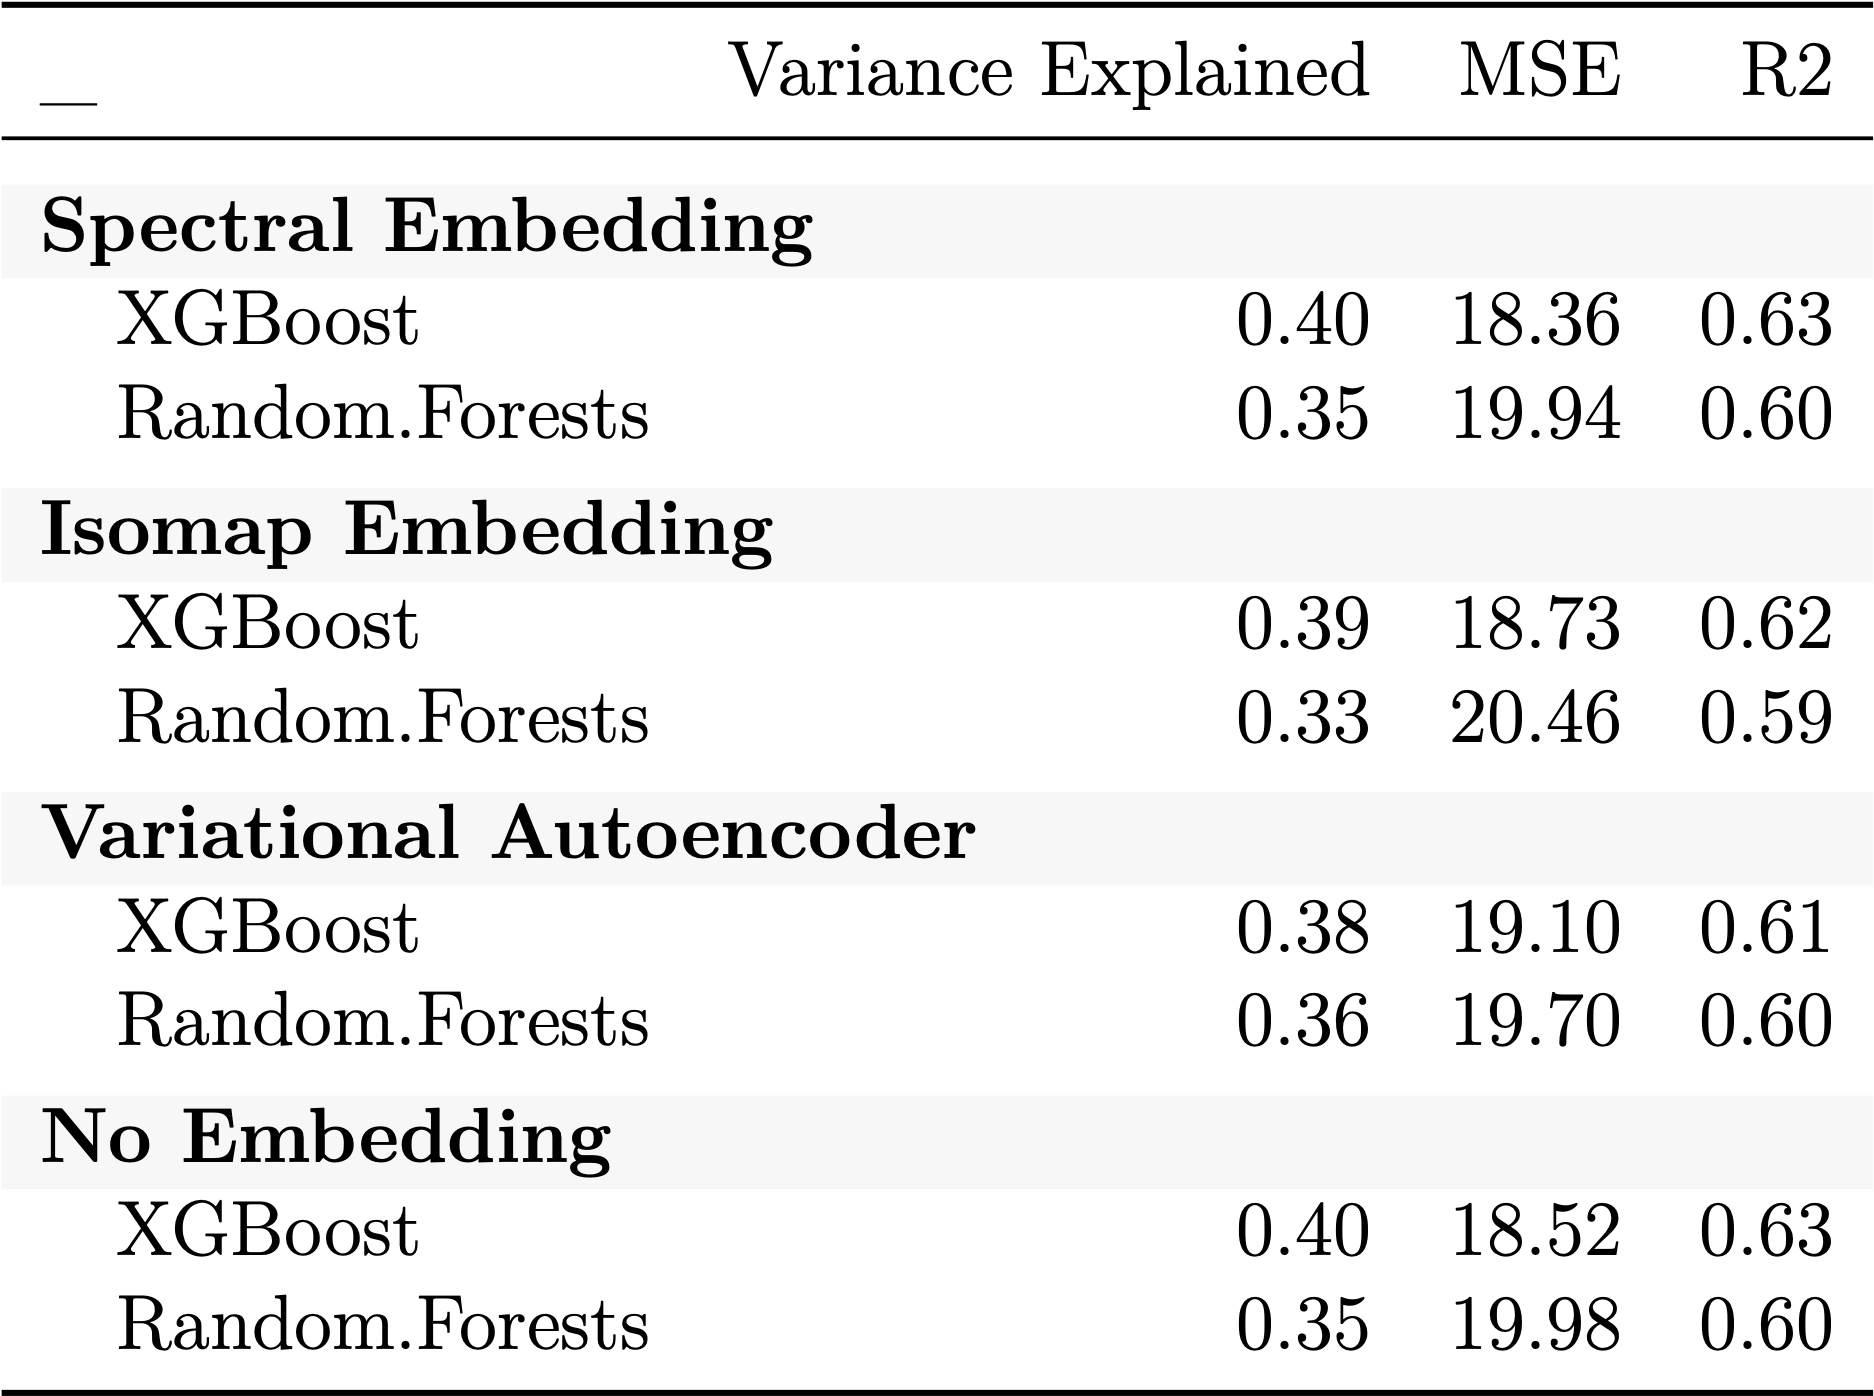
\includegraphics[scale=0.22]{../Figures/regression.png}
\end{center}
\caption{Regression}
\label{regression}
\end{figure}

\section{Conclusion}
\label{conclusion}

Our inquiry shows that it is possible to learn about citation count from this data. However, it is also  clear that the majority of the signal comes from non-textual features, the data and journal of publication were much more predictive. This result is not conclusive though. Since our data are a subset of the total literature available on coronaviruses, our features designed to capture the relationship to other work may be impacted. This problem may also lead to inflated importance of underrepresented journals. If a journal is only represented a handful of times with highly cited papers, this may inflate the journal's importance if the papers unaccounted for have low citation counts. For this reason, it would be interesting to further this modeling attempt to include analysis that has already been conducted on the entire body of works for each author and journal.  

Taking this into account, it is likely that our text analysis and embedding techniques are not well suited to this task. Typically this type of work deals with disparate fields of study, while this inquiry looks at a set of academic papers focused on closely related subjects. This inherit similarity makes it more difficult for topic modeling and document vectorization techniques to separate the papers.

While our current models performed moderately well, we believe using tree based predictive modeling in combination with embedded texts has more promise on a more diverse set of papers. Interesting further research would include testing these methods on a more complete body of coronavirus literature and on papers from a wider range of academic fields. 

\newpage
\subsubsection*{References}

\small{
[1] Allen Institute For AI. “COVID-19 Open Research Dataset Challenge (CORD-19).” Kaggle, CDC, 25 Apr. 2020, www.kaggle.com/allen-institute-for-ai/CORD-19-research-challenge.

[2] Yan, Rui \& Tang, Jie \& Liu, Xiaobing \& Shan, Dongdong \& Li, Xiaoming. (2011). Citation count prediction: Learning to estimate future citations for literature. {\itInternational Conference on  Information and Knowledge Management, Proceedings} 1247-1252. 10.1145/2063576.2063757. 

[3] J. Hirsch. An index to quantify an individual’s scientific
research output. Proceedings of the National Academy of
Sciences of the United States of America, 102(46):16569,
2005.
}


\end{document}
